%\documentclass[12pt,twoside]{report}
\documentclass[12pt]{report}
% note that the document can be single or double sided.
\usepackage{suthesis-2e}

\usepackage{graphicx}
\usepackage{psfig}
\usepackage{epsfig}
\usepackage{subfigure}
\usepackage{algorithm}
\usepackage{float}
\usepackage[dvips]{color}

\usepackage{mathrsfs}
\usepackage{amsfonts}
\usepackage{amssymb,amsmath}
\usepackage[includemp,body={398pt,550pt},footskip=30pt,%
            marginparwidth=60pt,marginparsep=10pt]{geometry}

%\documentclass[11pt,a4paper,english,etoc,normalcite,sloppy]{zjuthesis}
%\definecolor{dgreen}{rgb}{0,.6,0}
%\newcommand\comments[1]{\textcolor{blue}{#1}}% my comments
%\renewcommand{\baselinestretch}{1.5}
%\input{preamble}


%\includeonly{
%body/Introduction,
%body/ConAirOverview,
%body/Design
%%body/RelatedWork,%
%%body/ModelingSS,
%%body/PropertiesOSS
%%body/Experiments,%
%%body/Conclusion % 
%}

\usepackage[normalem]{ulem}
\usepackage{subfigure}
\usepackage{cite}


\DeclareMathOperator*{\argmax}{argmax}

\begin{document}
%type of this report
\reporttype{Software Testing Final Project Report}

%%which department you are reporting to
\department2report{School of Engineering}

%the name of your unversity
\reportUniversity{University of Texas at Austin}

\title{ConAir: A Concurrency Bug Recovery Tool}
%\ctitle{Xiaoyong WEI}
\author{Shiyu Dong, Xuebin Yan}

%the name of your department
\dept{Electrical and Computer Engineering}

%the name of your supervisor
\principaladviser{Sarfraz Khurshid}

\submitdate{May 3,2014}



\pagenumbering{roman}

    \beforepreface
\prefacesection{Abstract}

Multimedia-based ontology construction and reasoning have recently
been recognized as two important issues in video search,
particularly for bridging semantic gap. The lack of coincidence
between low-level features and user expectation makes concept-based
ontology reasoning an attractive mid-level framework for
interpreting high-level semantics. In this report, we propose a
novel model, namely ontology-enriched semantic space (OSS), to
provide a computable platform for modeling and reasoning concepts in
a linear space. OSS enlightens the possibility of answering
conceptual questions such as a high coverage of semantic space with
minimal set of concepts, and the set of concepts to be developed for
video search. More importantly, the query-to-concept mapping can be
more reasonably conducted by guaranteeing the uniform and consistent
comparison of concept scores for video search. We explore OSS for
several tasks including concept-based video search, word sense
disambiguation and detecor fusion. Our empirical findings show that
OSS is a feasible solution to timely issues such as the measurement
of concept combination and query-concept dependent fusion.

    \afterpreface



%\input{acknowledgement}



%\listoffigures
%
%\listoftables

%\mainmatter


\graphicspath{{figures/}}
\pagenumbering{arabic} \setcounter{page}{1}
\chapter{Introduction}


\section{Background}
Information explosion is a term that describes the rapidly
increasing amount of published information and the effects of this
abundance of data. As the amount of available data grows, the
effective and efficient management of the information becomes more
difficult, leading to information overload or information fatigue.
The explosion problem of video data, in particular, posts more
technical challenges due to the fact that audio-visual features are
unorganized and unordered in nature. Video retrieval, aiming to mine
and search semantic knowledge from an over-abundance of video
dataset, has drawn increasing attentions from both extant web search
engines (e.g., Yahoo!, Google and so on) and scientific researchers.
However, the video usually carries a versatile semantic message
which has immediate meaning for a human. But for a computer, it is
far from the truth. This discrepancy between the machine computable
low-level features and its semantic interpretation by human subjects
is commonly referred to as the \emph{semantic gap}
\cite{ArnoldW.M.Smeulders:IEEETPAMI:2000}. Bridging semantic gap has
long been recognized as a key factor in enabling semantic-based
video retrieval.

Early efforts aiming to bridge the semantic gap focused on the
feasibility of mapping low-level features, e.g. color, pitch and
texture, directly to high-level semantic concepts such as commercial
\cite{R.Lienhart:IEEECMCS:1997}, nature \cite{J.R.Smith:IEEEMM:1997}
and baseball \cite{Y.Rui:ACMM:2000}. Many dedicated detectors have
been developed for this intuitive purpose, which map low-level
features to single semantic concept based on simple decision rules.
The detector-specific-approaches, however, become impractical and
intractable with the demand of large-scale automatic annotation of
video archives. It is almost impossible to develop a dedicated
detector for each possible concept, as there are just too many
concepts. Instead of developing concept-specific detectors, a recent
trend has therefore been shifting to develop generic detectors.
Specifically, with a set of concept-specific training examples,
generic detectors are trained separately with single approach
without considering concept-specific knowledge
\cite{MilindR.Naphade:IEEEICOME:2000,A.Amir:TRECVID:2003,C.G.M.Snoek:NISTTRECVID:2005}.
This has enlightened the possibility of developing large-scale
concept detectors, ending up a multimedia ontology suitable for both
video annotation and search.

The core of generic-based approaches mainly relies on the paradigm
of supervised learning \cite{CeesG.M.Snoek:ACMMM:2006}. The major
limitation, nevertheless, is the need of large amount of labeled
examples for training. The labeling of multimedia data is generally
a labor intensive, subjective and erroneous process. The researchers
have indeed looked forward a large shared annotation dataset for
concept detector learning. To cope with the demand, initiated by Lin
et al. \cite{C.Y.Lin:TRECVID:2003}, a common annotation effort was
recently started for the TREC Video Retrieval Evaluation (TRECVID
Workshop) 2005 benchmark. It has yielded a large accurate set of
groundtruth including a lexicon of 39 concepts
\cite{M.R.Naphade:2005}. Driven by this effort, various sets of
annotated concepts, such as Medmill's 101 machine-learned detectors
\cite{CeesG.M.Snoek:ACMMM:2006} and the recent collaborative
undertaking development of Large-Scale Concept Ontology for
Multimedia (LSCOM) \cite{Milind.Naphade:IEEEMM:2006}, have become
publicly available.

However, such a widely collaborative annotation effort, with such a
large amount of shared groundtruth, can never reach the richness of
human-know vocabularies. New concepts and new examples will have to
be annotated, when we face any new domain. More seriously, different
people tend to use different terms in annotating the same concept
during labeling, resulting in label ambiguity. Even for the same
user, he/she will trend to use different terms in different context.
To deal with this problem, ontologies
\cite{C.Fellbaum:1998,H.Liu:BTTJ:2004} were developed to structure
terms employed by user, which can make descriptions more consistent.
Exploiting ontology on video domain can embed the inherently
uncertain tagging, generated either by machine or human, in a
semantically rich context. With the multimedia ontology, we can
disambiguate various interpretations and find concepts that are more
general and useful for retrieval. As the video domain is broad and
in practice contains any topic, a large and domain independent
ontology is necessary.

\section{Ontology and Multimedia Ontology}
In philosophy, ontology is the study of the kinds of things that
exist. Ontologies are often said, colorfully,``to carve the world at
its joints". In information science, however, it is unrealistic,
when we realize that the world is too big to be carved. What we say
ontology is therefore referred to domain ontology, which describe
the body knowledge of a domain. Different from traditional domain
knowledge, an ontology analysis clarifies the structure of knowledge
by identifying the basic conceptualizations needed to talk about all
instances, recognizing their types, and relating the topology to
additional constraints. A well-structured knowledge representation
is easy to be shared with others who have similar needs in that
domain, thereby eliminating the need for replicating the
knowledge-analysis process. Shared ontologies can thus form the
basis for domain-specific knowledge-representation languages. In
contrast to the previous generation of knowledge-representation
languages (e.g KL-One \cite{R.J.Brachman:CS:1985}), these languages
are content rich; they have a large number of terms that embody a
complex content theory of the domain
\cite{B.Chandrasekaran:IEEEIS:1999}.

The current interest in ontologies come from the alternation of
focus between content theories and mechanism theories. Many
mechanisms, such as rule systems, frame languages, neural nets,
fuzzy logic, constraint propagation, or unification, are proposed as
exciting secret of making intelligent machines. With such wonderful
mechanisms, however, we cannot do much without a good content
theory. Moreover, we often recognize that once a good content theory
is reached, many different mechanisms might be used equally well to
implement effective systems, all using essentially the same content
\cite{B.Chandrasekaran:IEEEE:1994}. Ontologies are quintessentially
content theories. Thus far, they have played important roles in
information systems, natural language understanding (NLU) and
knowledge-based systems. In the domain of multimedia, ontology is
regarded as an emerging, yet natural, tool to bridge the semantic
gaps as a result of annotation ambiguity due to fuzziness of
audio-visual information. Ideally, ontology should be able to deal
with the richness of natural vocabularies, not only in textual but
also audio-visual domain.

Given the term Multimedia Ontology, people might usually refer to
some standard controlled vocabularies and classification schemes for
multimedia. For example, MPEG-7 has standardized more than 140
classification schemes that describe properties of multimedia
content. Similarly, TGM-I provides a large thesaurus for cataloging
graphical material. There are several multimedia controlled
vocabularies available. However, these standard schemes have
received little attention from the multimedia research community,
mostly because many of the terms in these schemes are not suitable
for automated tagging. For example, the MPEG-7 Genre Classification
Scheme (urn:mpeg:mpeg7:cs:GenreCS:2001), which is used to classify
programs based on their content or subject matter, defines terms
such as``special events" and``remarkable people." The terms might be
useful for classifying multimedia content but do not lend them well
to automated extraction. Such subjective concepts also make it
difficult for two annotators to completely agree, which further
complicates this issue. This highlights the third critical
requirement for the multimedia concept ontology: the feasibility of
automated extraction \cite{Milind.Naphade:IEEEMM:2006}.

Multimedia ontology helps to identify the body classes, their
properties and the relationship between them. It will provide the
reasoning strategy a well-structured knowledge base. On the other
side, the reasoning strategy also has impact on the development of a
multimedia ontology. We could in fact explain this in a common
sense: how we build a thing is strongly related with how we use it,
and vice versa.

\section{Concept-based Video Search and Ontology Reasoning}
Recent applications of using multimedia ontology are mainly for
concept-based video search, as illustrated in
Figure~\ref{fg-semantic_gap}.
%
The sensory gap from user queries to raw data is bridged with a pool
of concepts enriched with general-purpose vocabularies, for
instance, from ontology (e.g., WordNet) and external information
(e.g., Internet). Based on such concepts, a set of concept detectors
is developed to represent the high-level semantics. The detectors
are automatically learnt with training examples described by
multi-modality features. Given a user query, the best set of
concepts that can describe the semantic of query is reasoned through
the vocabularies. A search list is then produced by ranking items
(e.g., shots) according to their signal responses to the selected
concept detectors.
%
\begin{figure}[t]
\centering
\includegraphics[width=0.8\textwidth]{semantic_gap.eps}
\caption{General framework of concept-based video retrieval.}
\label{fg-semantic_gap}
\end{figure}
%

Under the concept-based retrieval framework as depicted in
Figure~\ref{fg-semantic_gap}, an apparent issue is that, given the
concept set, the mapping ambiguity between queries and concepts
needs to be carefully resolved. A common solution is to consider the
mapping through ontology reasoning
\cite{CeesG.M.Snoek:IEEETM:2006,Anthony.Hoogs:CVPR:2003,Alejandro.Jaimes:ICOIVR:2003,Yi.Wu:IEEEICOME:2004,M.R.Naphade:2005},
or more precisely selecting the concepts which minimize the
linguistic distance with query terms. The mapping is normally done
with the shared knowledge topology such as WordNet
\cite{C.Fellbaum:1998}. A fundamental question is: whether the
ontology reasoning can provide a common ground for the consistence
reasoning of concept similarities?
%
\begin{figure}
 \centering \subfigure[]
{\includegraphics[width=0.48\textwidth]{cfo.eps}\label{fig:cfo}}
 \centering \subfigure[]
{\includegraphics[width=0.48\textwidth]{OSS.eps}\label{fig:oss}}
%\subfigure[]
%{\includegraphics[width=0.24\textwidth]{os2mode.eps}\label{fig:os2}}
\caption{Reasoning with (a) ontology, reasoning is done in a
subgraph without a global view of the whole structure, (b) OSS,
concepts are projected into the space according to their relations
with selected vantage (basis) concepts.}\label{fig:CFO_OSS}
\end{figure}
%
Take Figure~\ref{fig:CFO_OSS}(a) as an example, let concepts $a$ to
$e$ as children and $v_1$ to $v_3$ as ancestors. Using ontology
reasoning approach such as Resnik \cite{Philip.Resnik:IJCAI:1995}
which measures similarity of two concepts with Information Content
(IC) \cite{Philip.Resnik:IJCAI:1995} of their nearest common
ancestor, the concept pairs $(a,b)$ and $(a,c)$ could have the same
similarity equals to IC of $v_1$, although $(a,c)$ sharing another
ancestor $v_2$ and intuitively should be more alike. In this case,
supposing $a$ is a query item, concept selection is hard to be made
between $b$ and $c$. On the other hand, the similarity scores of
$(d,e)$ and $(a,b)$ cannot be reasonably compared as they reside in
different parts of the ontology which carry different statistic and
structural information.
%
In brief, the reasoning is {\em locally} determined in a subgraph
without a global ontological view. Such mapping strategy indeed
causes the similarity scores of query terms and concepts not
directly comparable, resulting in less meaningful matching when
finding the ``best concepts'' to interpret query semantics.

\section{Ontology-enriched Semantic Space}
In this report, we propose a novel model called Ontology-enriched
Semantic Space (OSS) to enable the uniform and \emph{global}
comparison of concept pairs by providing a {\em computable}
platform. With reference to Figure~\ref{fig:CFO_OSS}(b), the
semantic space is represented as a linear space spanned with a set
of concepts enriched with ontology knowledge. These concepts of OSS
can be viewed as the ``vantage'' points
\cite{RobertoF.Santos.Filho:ICDE:2001,CaetanoTraina.Jr.:VLDB:2007}
\cite{Malcolm.Slaney:ICME:2002,A.Berenzweig:ICME:2003,Jules.Vleugels:PR:2002}
of the original ontology space. Supposing the ancestors $v_1$ to
$v_3$ of Figure~\ref{fig:CFO_OSS}(a) are selected as the vantage
concepts of OSS, then one can linearly project the concepts $a$-$e$
to the metric space according to their ontological relation with the
selected vantage concepts through conventional ontology reasoning.
Such framework indeed sights several opportunities. First, the
vantage concepts provide a high coverage of semantic space, and are
probably the ones that should be developed if they are feasible to
be built with the current technology. Secondly, in contrast to the
examples in Figure~\ref{fig:CFO_OSS}(a), the space guarantees
\emph{global} consistency in comparing the concept pairs like
$(a,b)$, $(a,c)$ and $(d,e)$.

An intuitive explanation of OSS is that the space is linearly
constructed to model the available set of concepts. The expressive
power of OSS is linguistically spanned with a set of vantage
concepts, which is easier to generalize, not only to the available
concept detectors but also to the unseen concepts.

%However, some of the vantage concepts of OSS may have inter-concept
%correlation, which causes their corresponding vectors are not
%strictly orthogonal to each other. This will bias the measurement of
%similarity. To solve this problem, we further model the
%orthogonality of semantic space, resulting in an Orthogonal
%Ontology-enriched Semantic Space ($OS^2$). In contrast to OSS,
%$OS^2$ performs spectral decomposition to transform the semantic
%space into a novel space with orthogonal base. With reference to
%Figure~\ref{fig:CFO_OSS}(c), the base ($B_1$, $B_2$ and $B_3$) in
%$OS^2$ are not formed by the real concepts. They are, however,
%linear combinations of basis concept vectors of OSS, and are more
%powerful in terms of expressive and generalization abilities for
%having the orthogonal property which optimally covers the semantic
%space. Thus a more consistent way of comparing concept similarity
%scores can be guaranteed in $OS^2$.

\section{Organization of This Report}
With OSS, we explore several search related tasks including concept
selection and detector fusion in this report. The major
contributions of our works are briefly summarized as follows:
%
\begin{itemize}
\item
{\em Scalability}: Building detectors for all concepts is impossible
and not necessarily \cite{A.Hauptmann:CIVR:2007,W.H.Lin:ICME:2006}.
A practical question is which detectors should be developed given
the information at hand. Compared to recent works in
\cite{W.H.Lin:ICME:2006}, OSS provides another novel view of
selecting concepts which have higher generalization ability in query
answering.


\item
{\em Query-concept mapping}: With OSS, the mapping is no longer a
local similarity comparison. Global consistency is ensured so that
the selection of concepts becomes meaningful.


\item
{\em Query disambiguation}: User queries are mostly ambiguous. We
explore OSS to predict the search intention by finding the exact
senses of query terms.
\end{itemize}

The remaining chapters are organized as follows.
Chapter~\ref{chp:related_work} briefly describes the current
state-of-the-art about multimedia ontology and concept-based video
search. Chapter~\ref{chp:modelingSS} presents the main idea of
modeling and constructing OSS. Chapter~\ref{chp:properties} analyzes
the properties of OSS. Finally, Chapter~\ref{chp:experiments}
presents experiments and Chapter~\ref{chp:conc} concludes this
report.

\chapter{ConAir Overview}
\label{chp:Overview}
\section {Two observations}
The design of ConAir is based on two ovservations:
\begin{itemize}
\item
Roll back a single thread is sufficient to recover from most concurrency-bug failures.
\item
Reexecute an idempotent region is sufficient to recover from many concurrency-bug failures.
\end{itemize}
\section{Observation I}
For most concurrency bugs, reexecuting one failing thread is sufficient to fix bugs.In the following part, most common concurrency bugs will be discussed separately:\\
\subsection{Recovering atomicity-violation bugs}
Atomicity violations contribute to about 70 \% of real-word non-deadlock bugs[].For read and write operations, there are four kinds of atomic violation operations, including Read after Write (RAW), Read after Read (RAR), Write after Read (RAW) and Write after Write (WAW). 
\begin{figure}
\begin{minipage}[t]{0.52\linewidth}
\centering
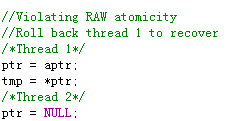
\includegraphics[width=\textwidth]{body/RAW.png}
\caption{RAW atomic violation}
\label {RAW}
\end{minipage}%
\begin{minipage}[t]{0.52\linewidth}
\centering
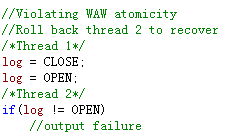
\includegraphics[width=\textwidth]{body/WAW.png}
\caption{Violating WAW atomicity}
\label{WAW}
\end{minipage}
\end{figure}

\begin{figure}
\begin{minipage}[t]{0.52\linewidth}
\centering
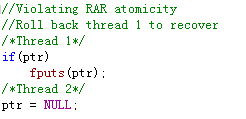
\includegraphics[width=\textwidth]{body/RAR.png}
\caption{RAR atomic violation}
\label {RAR}
\end{minipage}%
\begin{minipage}[t]{0.52\linewidth}
\centering
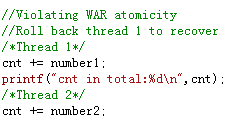
\includegraphics[width=\textwidth]{body/WAR.png}
\caption{Violating WAR atomicity}
\label{WAR}
\end{minipage}
\end{figure}
As in Figure~\ref{RAW}, in thread 1, a global pointer is set to point to aptr and then, dereference it and give the value to a local variable tmp. In thread 2, the global pointer is initialized to NULL. Consider the situation that the first sentence of thread 1 is executed and then thread 2 is executed. When ptr is dereferenced and give its value to tmp, segamentation fault happens. In this case, roll back thread 1 until thread 2 finishes and do the given value part. The bug can be fixed.\\
As in Figure~\ref{WAW}, if thread 2 happens before the end of thread 1, error happens. In this case, rolling back thread 2 can fix the bug.\\
As in Figure~\ref{RAR} and Figure~\ref{WAR}, still rolling back one thread can fix the possible concurrency bugs. In general, for atomic violation bugs, rolling back one thread is sufficient to fix them.
\begin{figure}[t]
\centering

\includegraphics[width=0.7\textwidth]{body/order_violation.png}
\caption{Order violation bug}
\label{order violation}
\end{figure}
\subsection{Recovering order-violation bugs}
Another kind of concurrency bug is called order-violation. That is one thread is required to be finished before another one. For example, in Figure~\ref{order violation}, A is required to finish before B. In this case, roll back B until A finishes can fix the bug.
\subsection{Rocovering deadlock bugs}
A very common concurrency bug in multi-thread programming is deadlock problem. As in Figure~\ref{deadlock}, thread A holds lock 1, thread B holds lock 2 and thread C holds lock 3. A still wants lock 2, while it's held by B. So A is blocked. Similar situation happens in B and C. In this case, roll back any thread can fix deadlock. If roll back B, B releases lock 2, so that C can finish and release lock 3 and 2. Then B can finish. Finally, A can get all resource it wants and finish itself.
\begin{figure}[t]
\centering
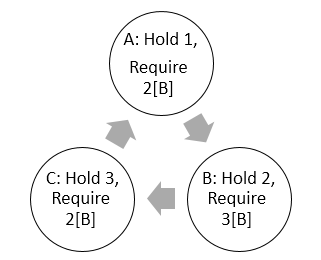
\includegraphics[width=0.7\textwidth]{body/deadlock.png}
\caption{Deadlock}
\label{deadlock}
\end{figure}

\section{Observation II}
For observation II, it indicates that roll back certain area of one thread is sufficient to fix bugs and that area is defined as idempotent region.\\
\textbf{Idempotent region}:a code region that can be reexecuted for any number of times without changing the program semantics.\\
It should end before the failing point because it is meaningless to roll back the error part. Besides it, the idempotent region should not contain any writes to shared variables. If it is, roll back it will continously change a global variable, which is unwanted by users. Furthermore, it will not contain any I/O operations. According to investigation, only 15 \% concurrency bugs contain I/0 operation. In order to guarantee the performance of ConAir, I/O operation is eliminated from idempotent region. Also, it should not contain any writes to local variables that could cause incorrect execution. This rule is also added to guarantee the correnctness of the ConAir. Some local variables, such as static ones is initialized once and changed extends for the entire run of the whole program. If it is included in the idempotent region, potentially incorrect output may happen.\\
All rules are set to guarantee the correctness and performance of the usage of ConAir. Above all, the working principle of the ConAir is to roll back a single thread (failing thread) with its idempotent region.

 
\chapter{Design and Implementation of ConAir}
\label{chp:Design}
According to the working principle of ConAir, there are three main challenges of the design of ConAir. 
\begin{itemize}
\item
How to decide the failing point of the program
\item
How to find the idempotent region of the thread
\item
How to realize roll back step
\end{itemize}

\chapter{Infrastructure}
In this chapter we will discuss our infrastructure setup for building and
running ConAir, and the toolchain of using the ConAir tool.

\section{Infrastructure Setup}
One of the standards that was mentioned previously to evaluate the tool is
Compatibility, which means the tool should have no OS/hardware modification.
When we try to build and run the ConAir tool, however, we find out that although
it does not require any OS/hardware modification, it has very strong requirement
to the OS and corresponding software installed.

We make many effort in order to make Conair compile and run. For example, We try
four different versions of Linux: Ubuntu 12.04 x64, Ubuntu 12.04 x86, the
Lonestar Cluster of UT, as well as CentOS 5.9. The first two are the OS that we
have as a virtual machine. None of them work perfectly. Then we ask the
author and they provide us the specific OS version that they use. Then we try
Lonestar Cluster which has an OS pretty similar to the one that the author
provides, but we do not have the previlidge to install the required runtime
library. Finally we tried CentOS 5.9 which is exactly the same as the author
suggests, but we still cannot fix the compatibility issue (missing GLIBCXX\_3.4.9
and GLIBC\_2.7).

We also try different versions of LLVM, llvm-gcc and gcc. Specifically, we try
two versions of LLVM, llvm-2.8 and llvm 2.9; we try three versions of llvm-gcc:
the binary of llvm-gcc-4.2-2.8, binary of llvm-gcc-4.2-2.9, and llvm-gcc-4.2-2.8
built from source code; also we try five different versions of gcc: 4.7.3,
4.6.3, 4.4.3, 4.2.1 and 4.3.1 from source. For each try we do our best to remove
any compilation or dependency issue, and we try many combination between
different OS, LLVM, llvm-gcc and gcc. This process is very tedious and it take
more than 50\% of our time for this project. However, although we try very hard
we still cannot find a combination that is perfectly working. The main problem
we face is that the front end of LLVM cannot treat floating point global
variables appropriately. We believe that is because the version of LLVM we use
is too old, but ConAir does not support newer version of LLVM.

Fortunately, although we have the above issue, for normal multithread programs
without floating points we are able to make ConAir compile and run. Therefore we
can still do some experiments to demonstrate the effect of ConAir. We will show
our experiment results in section~\ref{sec:experiment}

\section{Toolchain}
There are several steps needed to make ConAir work, and
Figure~\ref{fig:toolchain} shows the structure of the ConAir ToolChain.
\begin{figure}
\centering
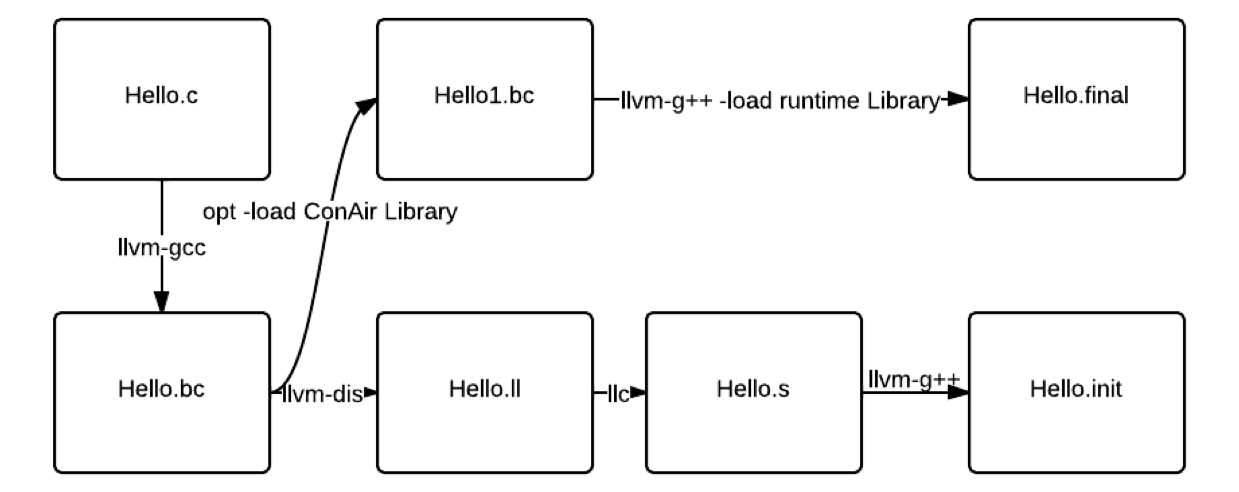
\includegraphics[width=\textwidth]{body/toolchain.png}
\caption{Toolchain of ConAir}
\label{fig:toolchain}
\end{figure}


\chapter{Experiment}
\section{ex1}

\chapter{Discussions and Future Work}
\section{diss}

\chapter{Related Work}
\label{chp:related_work} Despite the fact that bridging semantic gap
is simply an intuitive idea, it has taken almost a decade's research
effort. Various methodologies have been addressed so far, which
probably imply the difficulty and diversity of the problem domain.
In this chapter, we briefly review the existing approaches and
outline the major research challenges.

Traditional video retrieval methods assume that low-level features
correspond to the high-level semantic of queries. Features often
come from video associated textual resources such as closed captions
and transcript generated by automatic speech recognition (ASR)
\cite{M.Brown:ACMM:1995,B.Adams:TREC:2002}. In addition, some visual
features, like shape in \cite{A.Del.Bimbo:IEEETPAMI:1997}, texture
in \cite{W.Ma:MS:1999}, color in \cite{Th.Gevers:IEEETIP:2000} are
extracted from images. Recent methods aiming to bridge the gap by
developing dedicate detectors using both text and image features,
were proposed in
\cite{R.Lienhart:IEEECMCS:1997,J.R.Smith:IEEEMM:1997,Y.Rui:ACMM:2000}.
These so called concept-specific detectors then face the problem of
scalability, which gives birth to generic detectors
\cite{MilindR.Naphade:IEEEICOME:2000,A.Amir:TRECVID:2003,CeesG.M.Snoek:ACMMM:2006}.
The biggest challenge of deriving a multimedia ontology based on
generic detectors is the demand of vocabulary size and training
sample. Both demands are driven by system usage and development
respectively. Naturally, increasing vocabulary size implies the need
for more training samples. Nonetheless, training data is always
limited while the size of natural vocabulary is numerically
uncountable. Towards this end, an ideal multimedia ontology should
have the capacity to extend knowledge with minimum incremental
update. Specifically, the ontology should have the ability of
inferring unseen vocabularies from the numerically limited
concepts/detectors through reasoning, with the assistant of external
resources such as Web.

\section{Concept Set}
The use of multimedia ontology for narrowing semantic gap has been
recognized as a vital direction to approach semantic based
retrieval. Current ontologies consider mainly the identifying and
inclusion of high-level concepts that are feasible to be detected
and useful for retrieval. Available concept sets for the
constriction of ontology or reasoning include the 1000-concept LSCOM
\cite{Milind.Naphade:IEEEMM:2006}, 101 concepts from MediaMill
concepts \cite{CeesG.M.Snoek:ACMMM:2006}, and 39 Lite-LSCOM by
TRECVID community benchmark \cite{M.R.Naphade:2005}. The 39 concepts
from TRECVID 2005 benchmark is the most popular one, including
concepts like``Face",``Person", and``Sports". Later on, MediaMill
extends it to a larger set of 101 concepts
\cite{CeesG.M.Snoek:ACMMM:2006}, in which some specific named person
are appended e.g.``G.Bush jr",``I.Allawi", and``T.Blair". As a
collaborative effort, LSCOM further enlarge the set to 1000 concepts
\cite{Milind.Naphade:IEEEMM:2006}, aiming to standardize multimedia
semantics. What set of semantic concepts should the community focus
on? It is still an ongoing research topic. However, the final goal
for the moment should be a set of appropriate size, suitable for
automatic tagging techniques. In this set, right concepts are
included, which form a basis of semantic space. Further unseen terms
could be easily represented respect to this basis.

\section{Existing Ontologies}
Ontology is a formulated and sharable knowledge base, believed to be
supplementing each other with mechanism theories. It is primarily
used in text retrieval. Distinguishing from traditional
keywords-based retrieval methods, the ontology makes the relation
between property values and agents explicit, telling which property
value is connected using which property to which element of the
subject mater \cite{A.Th.(Guus).Schreiber:IEEEIS:2001}. Consider
"chimpanzee under large tree." Reduced to keywords,``large" can
refer to the chimpanzee or the tree. The ontology provides relations
between the terms. Inheritance relation, for example, is very
important to control means to widen or constrain a query.

Bringing ontology to multimedia domain is a comparatively new
research topic; even several attempts have been made in recent
years. Starting form year 2003, Hoogs \cite{Anthony.Hoogs:CVPR:2003}
add semantics to visual detectors by establishing links with a
general-purpose ontology. In their methods, visual characteristics
taking information of scene and motion are attached terms in
Wordnet. Respecting to relation information from Wrodnet, Bayesian
method is employed to handle large uncertainties, sparse data and
prior knowledge.

At the same year, instead of making use of existing ontology,
\cite{Alejandro.Jaimes:ICOIVR:2003,Alejandro.Jaimes:IEEEICOME:2003}
proposed a semi-automatic method to construct multimedia ontology.
Their idea is to learn key concepts and relations from training
textual data by using a standard text mining tools implemented in
KAON \cite{A.Maedche:IEEEDEB:2002}. A rules-based reasoning is
performed on the semi-automatic constructed ontology. During the
constructing, however, too much human judgments are required to
determine the types of relations detected, e.g. properties or
inheritance.

Limited by the semantic gap, as we have seen, it is difficult to
link low-level features and high-level concepts together. Mezaris
\cite{Mezaris:IEEETCSVT:2004} expand their image ontology
\cite{Mezaris:ICIP:2003} to multimedia domain, in which an
intermediate level is set up aiming to bridge the low-level visual
features and high-level concepts. The intermediate level serves to
map digital low-level features to corresponding semantic ones, e.g.
color value between a predefined range will be mapped to``red" or
"blue" and so on. After the mapping, an image region will be
presented by series of higher feature like dominate color, shape,
and background/foreground. Then intermediate features will be used
to infer higher concepts in object ontology, which named but did not
be presented in their paper. In sense, this architecture seems
reasonable. However, in their work, it just provides filters
effectively eliminating some irrelevant annotation. The final
decision has to be made by user in a traditional relevance feedback
manner.

Instead of using complex ontology, Wu \cite{Yi.Wu:IEEEICOME:2004}
employed a simple hierarchical decision tree for
multi-classification. After constructing the each single concept
model independently, ontology-based concept learning improves the
accuracy of individual concept by considering the possible influence
relations between concepts based on predefined ontology hierarchy.
The main idea, called boosting factor, is to boost the precision of
concepts by taking influences from more reliable ancestors. By the
Shrinkage theory \cite{Andrew.McCallum:ICML:1998}, parameter
estimates in data-sparse children toward the estimates of the
data-rich ancestors in ways that are probably optimal under
appropriate condition \cite{Yi.Wu:IEEEICOME:2004}. New parameter
estimate of child could therefore be created by a linear
interpolation of all hierarchy nodes from the root to the child. The
simple hierarchy ontology used in this work, however, mixes
relations like hierarchical and homonym together. It might be a
disadvantage limiting the extending of this ontology.

Similar with the idea of Hoogs, MediaMill
\cite{CeesG.M.Snoek:IEEETM:2006} add semantics to detectors for
video retrieval. A set of machine learned concept detectors that are
enriched with semantic descriptions and semantic structure obtained
from WordNet. Their kernel of reasoning is based on semantic
similarity measurement. The detector having maximum similarity score
with given query will be regarded as the most relevant one. However,
the noisy information included in Wordnet sometimes causes the
unreliable of similarity measure, and affects the correct selection
of concepts.

Recently, Luo \cite{Hangzai.Luo:ACMMM:2006} proposed a
domain-dependent ontology for Medical Video Annotation, in which
some terms of medical are built for bridging the semantic gap. They
proposed a multi-task boosting framework to do the reasoning,
slightly similar with \cite{Yi.Wu:IEEEICOME:2004}. The ontology is
domain-dependent and has unproved capability to extend to other
larger domain.

The content of video, most of the time is unlimited, which will tend
to include information from all kinds of domain. This is a possible
difficulty of building ontology for multimedia. Neither by building
an entire ontology manually nor by extending a single ontology
including general knowledge, \cite{Huan.Wang:ACMM:2006} provides an
alternative way to build ontology for multimedia domain, combining
ontologies of different domains. In their work, they take advantage
of combing an animal domain ontology, a textual description ontology
and a visual description ontology together. Reasoning is made by an
existing system RACER \cite{Volker.Haarslev:ACMSIGIRR:2001}. This
method takes less effort to construct ontology and easy to be
extended. However, keeping the consistence between employed
ontologies might be a potential issue for it.

\section{Ontology Reasoning}
\label{sec:ontology_reasoning} To select appropriate
concepts/detectors,
\cite{Yu-Gang.Jiang:NISTTRECVID:2006,CeesG.M.Snoek:IEEETM:2006,Shih-Fu.Chang:NISTTRECVID:2005}
 proposed methods based on semantic similarity
\cite{Philip.Resnik:IJCAI:1995}, which indicates the relatedness of
two words by querying Wordnet. Concepts/detectors, which are most
related (have highest semantic similarity) with original query text,
are selected. Thus, semantic similarity, which is still an ongoing
research topic of linguistic computing, becomes the kernel of such
approaches. There exist several semantic similarity measures,
different in terms of whether they exploit the structure or
information content of ontologies. Among them, Resnik measure
\cite{Philip.Resnik:IJCAI:1995} is the most popular one which has
been employed by
\cite{CeesG.M.Snoek:IEEETM:2006,Shih-Fu.Chang:NISTTRECVID:2005}. In
\cite{CeesG.M.Snoek:IEEETM:2006,Tat-Seng.Chua:NISTTRECVID:2006},
they utilize both concept description and ontology for similarity
measure. During offline indexing, each concept is manually linked to
1-6 synsets of Wordnet based on the concept description. During
mapping, the matching between query terms and the linked synsets of
a concept are evaluated with Resnik measures. A best matched concept
is then found for semantic retrieval. In
\cite{Tat-Seng.Chua:NISTTRECVID:2006,Shi-YongNeo:ICOIVR:2006}, a
more sophisticated framework is proposed. Both query terms and
concept descriptions are Wordnet expanded. More importantly they
fuse the statically expanded lexical information with dynamic
correlation by calculating the time-dependent mutual information
from external news sources. Specifically, with the time sensitive
expansion, the co-occurrence terms are found from the external
sources and used to dynamically weight the importance of concepts
across time. The final similarity is fused jointly with Resnik
measure, time-dependent information, as well as the detection
confidence of concepts.

There indeed exist several measures for semantic measures, such as
LCH \cite{C.Leacock:1998}, HSO \cite{G.Hirst:1997}, WUP
\cite{W.Zhibiao:AMACL:1994}, RES \cite{Philip.Resnik:IJCAI:1995},
LIN \cite{Dekang.Lin:AMACL:1997}, JCN \cite{JayJ.Jiang:ICRCL:1997},
Lesk \cite{M.Lesk:AICSD:1986}, Gloss Vector (Vect)
\cite{Siddharth.Patwardhan:ACLWMSSBCLPT:2006} and Pairwise Gloss
Vector (VP) \cite{Siddharth.Patwardhan:ACLWMSSBCLPT:2006}. LCH, HSO,
and WUP use path length information, while the remaining utilize
information content (RES, LIN, JCN) and the definition of word sense
(Lesk, Vect, VP). With a hierarchical tree of an Ontlogy like
WordNet, denote $D$ as the depth and $I$ as the information content
of a concept, $L$ as the path length between two concepts, and
$p_{ij}$ as the common ancestor of concepts $c_i$ and $c_j$. $D$
indicates the specificity of a concept, the larger the more
specific. Intuitively, the longer the $L$ path length is, the more
two concepts are differ to each other. The information concept $I$
is a measurement of the volume of information contained in a
concept. The measures are defined as (Formula of HSO has not been
included for its complicity. Reader could refer to
\cite{G.Hirst:1997}.)
\begin{eqnarray}
LCH(c_i,c_j) & = & -\log \frac{L(c_i,c_j)}{2\delta}\\
WUP(c_i, c_j) & = & \frac{2 D(p_{ij})}{L(c_i,c_j)+2D(p_{ij}))}\label{eqn:wup} \\
RES(c_i,c_j) & = & I(p_{ij})\\
 LIN(c_i,c_j) & = & \frac{2 I(p_{ij})}{I(c_i)+I(c_j)} \\
 JCN(c_i,c_j) & = & \frac{1}{I(c_i)+I(c_j)-2I(p_{ij})}
\end{eqnarray}
where $\delta$ is the maximum depth of WordNet. The information
content is estimated based on the one-million-word Brown Corpus of
American English \cite{N.Francis:1982}. Lesk utilizes the number of
shared words (overlaps) in the definitions (glosses) of concepts.
Vect represents concepts as gloss vectors using the co-occurrence
information derived from glosses. The cosine similarity between
gloss vectors is used to measure the concept relatedness. VP is
basically similar to Vect, except in the way it augments the glosses
of concepts with adjacent glosses.

\section{Ontology-based Video Search}
While encouraged by the richness of ontology reasoning approaches,
the issue of building concept ontology for query-concept mapping
remains open and unsolved
\cite{S.F.Chang:NISTTRECVID:2006,C.G.M.Snoek:NISTTRECVID:2006,W.H.Lin:ICME:2006}.
Multimedia and visual based ontology construction has been
previously addressed in
\cite{CeesG.M.Snoek:IEEETM:2006,Anthony.Hoogs:CVPR:2003,Hangzai.Luo:ACMMM:2006,L.Hollink:ACMMM:2005}.
The construction mostly involves the manual mapping of visual
elements to textual concept entities provided by shared
vocabularies. In \cite{Anthony.Hoogs:CVPR:2003}, WordNet is extended
with visual tags describing properties such as visibility, motion
and frequency of occurrence. In \cite{L.Hollink:ACMMM:2005}, based
on WordNet and MPEG-7, a visual ontology is created by linking
visual and general concepts. In view of the richness of human
vocabularies and the need for domain experts in tagging or creating
links, the scalability of these approaches is still remain unclear.
A relatively straightforward approach is recently proposed in
\cite{CeesG.M.Snoek:IEEETM:2006} by directly attaching concept
detectors to WordNet synsets. The semantically enriched detectors
can thus utilize contextual information provided by WordNet.
%In addition to the ontologies built on the basis of
%general-purpose vocabularies, domain specific multimedia ontology is
%also investigated in \cite{}.
%In \cite{}, two animal domain
%ontologies are constructed separately for textual and visual
%descriptions. The study indicates that the ontologies are useful for
%image retrieval.
Different from the existing ontology construction
\cite{CeesG.M.Snoek:IEEETM:2006,Anthony.Hoogs:CVPR:2003,L.Hollink:ACMMM:2005},
our approach utilizes the concept inter-relatedness to construct an
ontology-enriched semantic space. The space is computable and more
viable for query-concept mapping, particularly for fusing the
outputs of multiple concept detectors.

Depending on the types (visual or text) of queries, the mapping from
queries to concepts can be performed with detectors
\cite{M.Campbell:TRECVID:2006} or resources such as ontology
\cite{Shi-YongNeo:ICOIVR:2006,CeesG.M.Snoek:IEEETM:2006,C.G.M.Snoek:NISTTRECVID:2006},
text description \cite{CeesG.M.Snoek:IEEETM:2006} or co-occurrence
statistic \cite{M.Campbell:TRECVID:2006,Shi-YongNeo:ICOIVR:2006}.
%
For queries with image or video examples, the responses of detectors
basically indicate the likelihood of corresponding concepts present
in queries. For instance, the best confident detector is selected
for search in \cite{CeesG.M.Snoek:IEEETM:2006}.
%
For text queries, the mapping is usually performed through ontology
reasoning.
% which includes two steps: word sense disambiguation (WSD)
%and concept selection. A popular algorithm for WSD is Lesk algorithm
%\cite{} which automatically extracts the actual sense of query
%terms.
Various ontology similarity measures introduced in
Section~\ref{sec:ontology_reasoning} could be directly employed for
computing the association between terms and concepts.
%Popular measures include Resnik \cite{Philip.Resnik:IJCAI:1995}, JCN
%\cite{JayJ.Jiang:ICRCL:1997} and WUP \cite{W.Zhibiao:AMACL:1994}
%which consider ontological properties such as the specificity and
%information content of a concept, and the linguistic path length
%between two concepts.
%
In addition to ontology reasoning, other approaches for mapping text
queries are to compare queries against the text descriptions
associated with concepts \cite{CeesG.M.Snoek:IEEETM:2006} or to
expand queries with related terms \cite{Shi-YongNeo:ICOIVR:2006}.
The expanded terms as well as their weights can be learnt from
training examples \cite{M.Campbell:TRECVID:2006} or external
information such as Internet \cite{Shi-YongNeo:ICOIVR:2006}.
%
Nevertheless, due to the difficulty of obtaining training examples,
particularly for cross-domain video search, corpus training is
generally not scalable.

A different strategy of query-to-concept mapping is via the
construction of semantic space or vector space for modeling
concepts. The pioneering work in
\cite{Apostol(Paul).Natsev:ACMSIGKDD:2004,JohnR.Smith:ICME:2003}
constructs a semantic space, or more precisely a vector space,
formed by the set of available concept detectors. In this space, a
retrieval item (e.g., shot) is represented as a vector of model
scores. The scores are computed based on the signal responses of the
detectors to the item. Contrasting to other approaches based on
ontology reasoning
\cite{CeesG.M.Snoek:IEEETM:2006,Xiao-Yong.Wei:ACMMM:2007}, no
specific detector is selected, but rather all detectors are involved
in the video search though each detector carries different weights.
In \cite{Xirong.Li:CIVR:2007}, the idea of tf-idf originated from
information retrieval, which weights the importance of a detector
according to its appearance frequency, is adopted to further improve
the search performance of vector space representation.
%

\section{Anchor Selection} OSS could be treated as a feature space,
in which each dimension represents the soft membership in one of the
selected anchor concepts. Seen this way, this work is related to
anchor space approaches such as
\cite{RobertoF.Santos.Filho:ICDE:2001,CaetanoTraina.Jr.:VLDB:2007}
for database indexing, \cite{Malcolm.Slaney:ICME:2002} for audio
retrieval and indexing, \cite{A.Berenzweig:ICME:2003} for
classification of music, \cite{Jules.Vleugels:PR:2002} for image
retrieval. The kernel of anchor-based approaches are, which and how
many concepts should be are selected as anchors. In
\cite{Malcolm.Slaney:ICME:2002,A.Berenzweig:ICME:2003,Jules.Vleugels:PR:2002},
anchors are simply determined by human assignment. More precisely,
\cite{RobertoF.Santos.Filho:ICDE:2001,CaetanoTraina.Jr.:VLDB:2007}
selects anchors by using a algorithm named``Hull of Foci" (HF),
which greedily search concepts which are mostly far apart in
original space as anchors. The number of anchors is determined with
\emph{correlation fractal dimension}, which is an approximation of
intrinsic dimension of a space and could be estimated by algorithms
like Box-counting
\cite{Christos.Faloutsos:ACMSIGMODICMD:2000,C.Traina.Jr.:XVBSDSBBD:2000}.

\section{Summary}
As discussed in this chapter, ontologies, as a potential direction
to bridge the gap in a more formal manner, facilitate problem
analysis and solution design. However, two issues remain unclear:
(1) which and how many concepts should be selected to develop
detector? (2) which semantic similarity measure is the best for
ontology reasoning, or more precisely, query-concept mapping?
Following chapters will answer these questions.


%\include{body/ModelingSS} 
%
%\include{body/PropertiesOSS}

%\include{body/Experiments}

\chapter{Conclusion}
\label{chp:conc} We have presented OSS as a new computable platform
for the uniform and consistent measurement of concept similarity and
combination. The platform, aiming at a high coverage of semantic
space with a minimal concept set, shapes the ways of modeling
concept inter-relatedness, while providing guideline for concept
development. To show the feasibility of OSS, we explore and
experiment search related tasks including word sense disambiguation
and concept selection. Our findings show that, due to the uniform
way of assessing similarity, OSS is a feasible solution for
large-scale video search and concept combination. Currently we
assume that OSS exists in a linear space for computational reason.
Whether a nonlinear space assumption is feasible for OSS remains an
unanswered issue that worths further investigation.

A useful resource currently not explored in OSS is the co-occurrence
statistics of concepts in video data. The statistics can be directly
utilized for basis concept selection, amending the semantic space
such that the co-occurred behavior can also be modeled. Under such
circumstance, the space is enriched with both ontology semantic and
statistics useful for video search. Developing the basis concepts in
this space as detectors could be more realistic since the statistics
indeed hint the utility and observability of the concepts.
%
In addition to positively correlated concepts, the set of negative
concepts (e.g., {\em indoor} versus {\em outdoor}) is also a useful
piece of information for fast pruning in video search as presented
in \cite{W.H.Lin:ICME:2006}. It is possible to have another
``negatively correlated'' semantic space, complementary to OSS, to
allow fast filtering one on hand, and effective searching on the
other hand. We will consider both aspects (co-occurrence and
negative correlation) as the future extension of OSS.
%


%\bibliographystyle{unsrt}
%\bibliography{Reference/reference}
%\mypub{My Publication Related to this
%Report}{unsrt}{Reference/mypub}

%\appendix
%\chapter{My Publications in the past year}
\begin{enumerate}
    \item \textbf{X.Y. WEI} and C. W. Ngo, ``Ontology-Enriched Semantic Space for Video Search", in \emph{ACM Multimedia} (ACM MM),
    2007.
    \item C. W. Ngo, Y. G. Jiang, \textbf{X.Y. WEI}, F. Wang, W. Zhao, H.-K. Tan, X. Wu, ``Experimenting VIREO-374: Bag-of-Visual-Words and Visual-Based Ontology for Semantic Video Indexing and Search``, in \emph{NIST TRECVID Workshop} (TRECVID),
    2007.
\end{enumerate}



\end{document}
